\chapter{Introduction}

\section{Context and Problem Definition}

Medication management is a high-stakes, complex process central to modern healthcare delivery. Its successful execution is critical for patient safety, yet it remains a major source of preventable adverse events. The landmark report "To Err is Human" by the Institute of Medicine brought global attention to the prevalence of medical errors, identifying them as a leading cause of morbidity and mortality \cite{kohn2000}. Subsequent research and initiatives by the World Health Organization have reinforced this reality, indicating that medication-related harm affects one in ten patients globally and that the associated costs are substantial \cite{who2017, who2022}.

A primary contributing factor to this problem is the fragmented nature of Health Information Technology (HIT) ecosystems within hospitals \cite{berwick2008}. Many healthcare institutions operate on a patchwork of legacy systems, often developed decades apart using disparate technologies \cite{kazemi2016}. This technological heterogeneity creates significant barriers to interoperability, resulting in information silos where critical patient data is not shared effectively between departments or professionals \cite{keasberry2017}. The workflow, which should be a seamless continuum from a physician's prescription to pharmaceutical validation and finally to nursing administration, is often interrupted by manual processes, verbal communications, and data re-entry, each step introducing a new opportunity for error.

\begin{figure}[htbp]
    \centering
    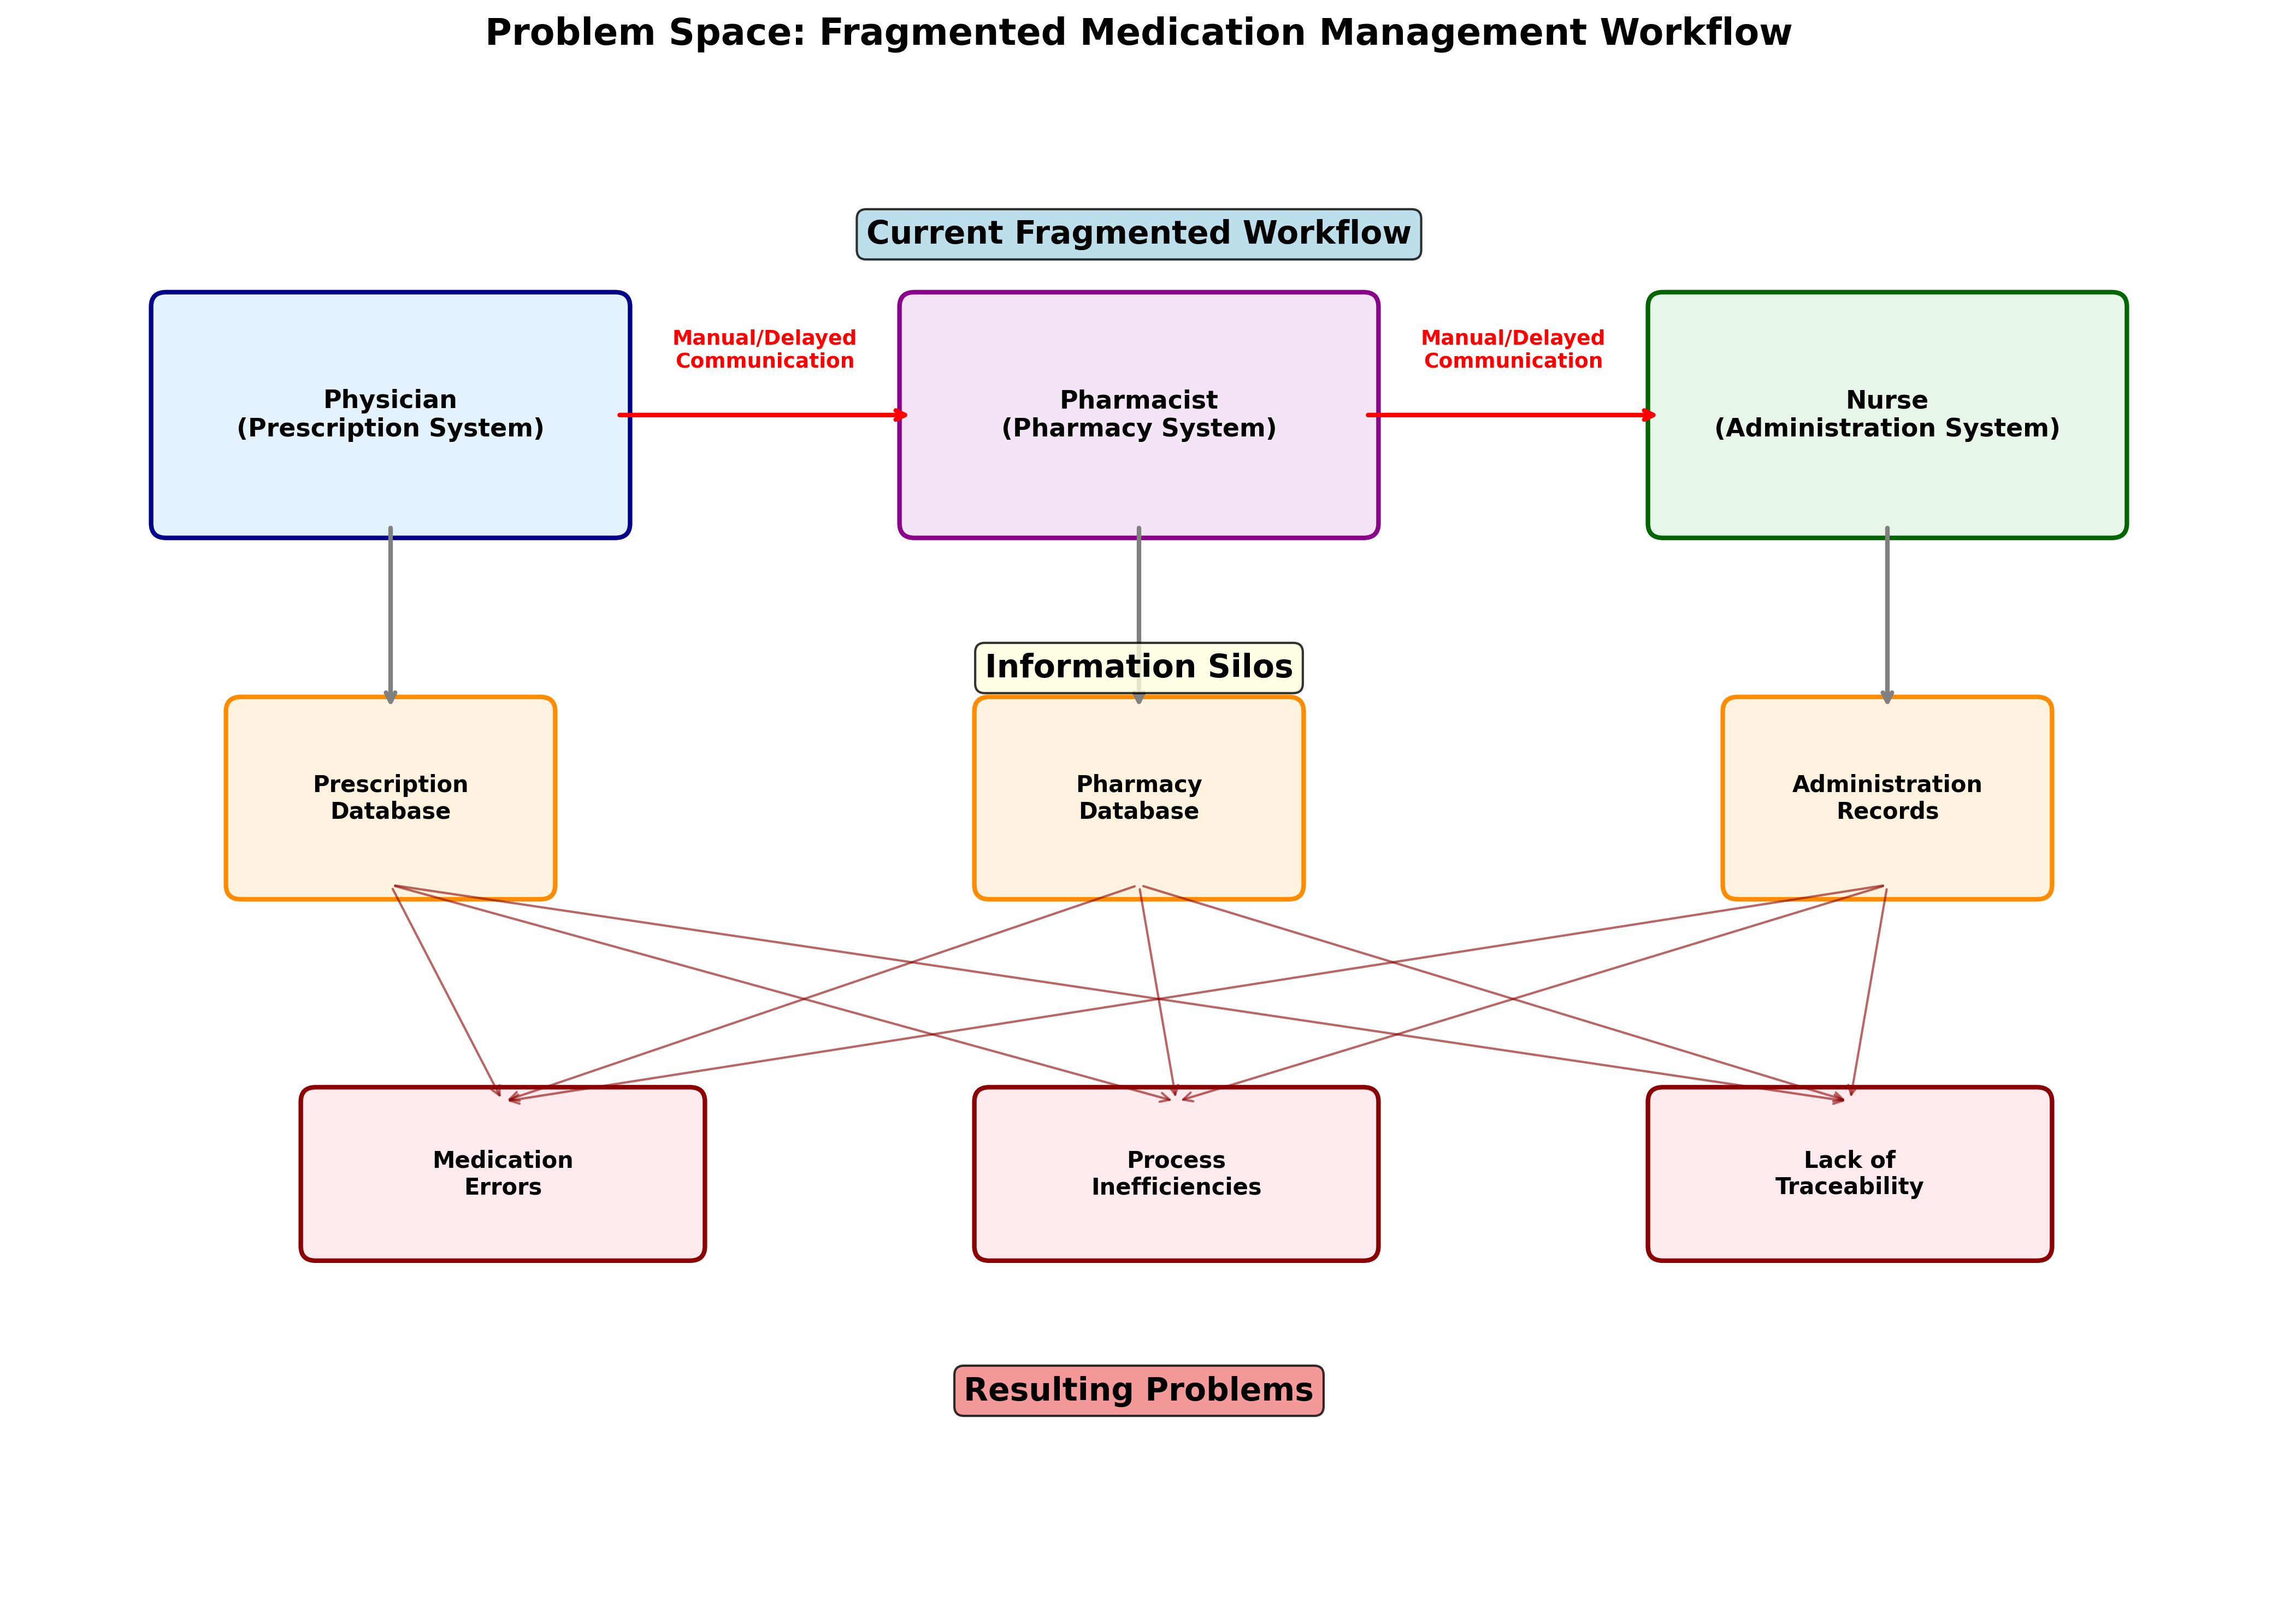
\includegraphics[width=0.9\textwidth]{images/generated/problem_space_diagram.png}
    \caption{Conceptual diagram of the problem space, illustrating the fragmented communication flow and resulting information silos that contribute to medication errors and operational inefficiencies.}
    \label{fig:problem_space}
\end{figure}

The Santa Casa da Misericórdia de Vila Verde (SCMVV) serves as a representative case study for these systemic challenges. Its core operations rely on the AIDA-PCE, a legacy system with significant limitations, including a non-intuitive interface, a lack of real-time clinical decision support (e.g., for drug interactions), and poor integration capabilities \cite{moss2015, bowles2020}. This environment compromises patient safety and hampers operational efficiency. This dissertation addresses these issues by detailing the design, development, and implementation of a modern, integrated medication management system aimed at creating a cohesive, safe, and efficient clinical workflow.

\section{Objectives}

The primary goal of this research is to develop and evaluate an integrated medication management system that optimizes the prescription, validation, dispensing, and administration processes at the SCMVV, thereby enhancing patient safety and operational efficiency.

To achieve this overarching goal, the following specific scientific and technological objectives were defined:

\subsection{Scientific Objectives}
\begin{enumerate}
    \item To analyze the impact of the integrated system on the rate of medication errors, quantifying the reduction in prescribing and administration faults.
    \item To evaluate the system's effect on clinical workflow efficiency by measuring key performance indicators, such as the time required for prescription and dispensing.
    \item To assess the usability and acceptance of the new system among clinical staff (physicians, pharmacists, and nurses) using established frameworks.
\end{enumerate}

\subsection{Technological Objectives}
\begin{enumerate}
    \item To design and implement a scalable and resilient backend based on a microservices architecture using Node.js and Java.
    \item To develop a robust, real-time clinical decision support engine for validating prescriptions against potential drug-drug interactions, allergies, and dosage errors \cite{belle2013}.
    \item To create a responsive and intuitive user interface using modern web technologies, such as React and Next.js, to streamline clinical tasks \cite{misra2023}.
    \item To ensure seamless, bidirectional integration with existing legacy systems, including the hospital's primary information system and pharmacy software, through a secure RESTful API layer \cite{mandl2020}.
    \item To establish a comprehensive audit trail for all medication-related activities, ensuring full traceability from prescription to administration \cite{european2016}.
\end{enumerate}

\section{Dissertation Structure}

This dissertation is organized into seven chapters, each addressing a specific aspect of the research.

\textbf{Chapter 1, Introduction,} provides the context for the research, defines the problem of medication management in fragmented hospital environments, and presents the scientific and technological objectives of the work. It concludes by outlining the structure of the document.

\textbf{Chapter 2, State of the Art,} offers a comprehensive review of the literature on hospital medication management systems, medication safety, emerging technologies such as Artificial Intelligence, and interoperability standards like HL7 FHIR. This review identifies the existing gaps that this research aims to address.

\textbf{Chapter 3, Work Plan,} details the project's methodology, including the phases of development, key tasks, timeline, and deliverables. It provides the strategic roadmap followed for the research and implementation process.

\textbf{Chapter 4, Methodology,} describes the architectural and technological choices made for the system's development. It elaborates on the microservices architecture, the specific technologies employed (React, Node.js, Oracle), the agile development approach, and the methods used for system evaluation.

\textbf{Chapter 5, Results,} presents the outcomes of the project. This includes a description of the final implemented system and a presentation of the quantitative and qualitative data gathered during its evaluation, such as error reduction rates, performance metrics, and user satisfaction scores.

\textbf{Chapter 6, Discussion,} interprets the results presented in the previous chapter, analyzing their implications in the context of the state of the art. This chapter also addresses the limitations of the study and reflects on the challenges encountered during the project.

\textbf{Chapter 7, Conclusion,} summarizes the key findings and contributions of the dissertation. It reiterates how the project met its objectives and concludes by proposing potential directions for future research and development in this domain. 